%%%%%%%%%%%%%%%%%%%%%%%%%%%%%%%%%%%%%%%%%%%%%%%%%%%%%%%%

\documentclass[12pt,a4paper]{article}% 文档格式
\usepackage{ctex,hyperref}% 输出汉字
\usepackage{times}% 英文使用Times New Roman
%%%%%%%%%%%%%%%%%%%%%%%%%%%%%%%%%%%%%%%%%%%%%%%%%%%%%%%%
\title{\fontsize{18pt}{27pt}\selectfont% 小四字号，1.5倍行距
	{\heiti% 黑体 
		Life Lab：AI Agent 实验平台简介}}%
%%%%%%%%%%%%%%%%%%%%%%%%%%%%%%%%%%%%%%%%%%%%%%%%%%%%%%%%
\author{\fontsize{12pt}{18pt}\selectfont\fangsong
	赵俊宇~~刘福康~~岳雨婷\\[3pt]
	\fontsize{10.5pt}{15.75pt}\selectfont\fangsong
	(中国科学技术大学~~~信息科学技术学院)}
%%%%%%%%%%%%%%%%%%%%%%%%%%%%%%%%%%%%%%%%%%%%%%%%%%%%%%%%
\date{}% 日期（避免生成日期）
%%%%%%%%%%%%%%%%%%%%%%%%%%%%%%%%%%%%%%%%%%%%%%%%%%%%%%%%
\usepackage{amsmath,amsfonts,amssymb}% 为公式输入创造条件的宏包
%%%%%%%%%%%%%%%%%%%%%%%%%%%%%%%%%%%%%%%%%%%%%%%%%%%%%%%%
\usepackage{graphicx}% 图片插入宏包
\usepackage{subfig}% 并排子图
\usepackage{subcaption}
\usepackage{float}% 浮动环境，用于调整图片位置
\usepackage[export]{adjustbox}% 防止过宽的图片
\usepackage{multirow}
\usepackage[table,xcdraw]{xcolor}
\usepackage{colortbl}
%%%%%%%%%%%%%%%%%%%%%%%%%%%%%%%%%%%%%%%%%%%%%%%%%%%%%%%%
\usepackage{bibentry}
\usepackage{natbib}% 以上2个为参考文献宏包
\setcitestyle{numbers,square}
%%%%%%%%%%%%%%%%%%%%%%%%%%%%%%%%%%%%%%%%%%%%%%%%%%%%%%%%
\usepackage{abstract}% 两栏文档，一栏摘要及关键字宏包
\renewcommand{\abstracttextfont}{\fangsong}% 摘要内容字体为仿宋
\renewcommand{\abstractname}{\textbf{摘\quad 要}}% 更改摘要二字的样式
%%%%%%%%%%%%%%%%%%%%%%%%%%%%%%%%%%%%%%%%%%%%%%%%%%%%%%%%
\usepackage{xcolor}% 字体颜色宏包
\newcommand{\red}[1]{\textcolor[rgb]{1.00,0.00,0.00}{#1}}
\newcommand{\blue}[1]{\textcolor[rgb]{0.00,0.00,1.00}{#1}}
\newcommand{\green}[1]{\textcolor[rgb]{0.00,1.00,0.00}{#1}}
\newcommand{\darkblue}[1]
{\textcolor[rgb]{0.00,0.00,0.50}{#1}}
\newcommand{\darkgreen}[1]
{\textcolor[rgb]{0.00,0.37,0.00}{#1}}
\newcommand{\darkred}[1]{\textcolor[rgb]{0.60,0.00,0.00}{#1}}
\newcommand{\brown}[1]{\textcolor[rgb]{0.50,0.30,0.00}{#1}}
\newcommand{\purple}[1]{\textcolor[rgb]{0.50,0.00,0.50}{#1}}% 为使用方便而编辑的新指令
%%%%%%%%%%%%%%%%%%%%%%%%%%%%%%%%%%%%%%%%%%%%%%%%%%%%%%%%
\usepackage{url}% 超链接
\usepackage{bm}% 加粗部分公式
\usepackage{booktabs}
\usepackage{longtable}% 长表格
\usepackage{supertabular}% 跨页表格
\usepackage{algorithm}
\usepackage{algorithmic}
\usepackage{changepage}% 换页

\usepackage{listings}
\lstset{
    basicstyle=\ttfamily\small,
    numbers=left,
    numberstyle=\tiny\color{gray},
    stepnumber=1,
    backgroundcolor=\color{gray!8},
    frame=single,
    rulecolor=\color{black!30},
    tabsize=2,
    breaklines=true,
    captionpos=b,
    showstringspaces=false,
    keywordstyle=\color{blue},
    commentstyle=\color{green!50!black},
    stringstyle=\color{purple},
    escapeinside={(*@}{@*)},
    columns=fullflexible,
    extendedchars=true,
    inputencoding=utf8
}
%%%%%%%%%%%%%%%%%%%%%%%%%%%%%%%%%%%%%%%%%%%%%%%%%%%%%%%%
\usepackage{enumerate}% 短编号
\usepackage{caption}% 设置标题
\captionsetup[figure]{name=\fontsize{10pt}{15pt}\selectfont Figure}% 设置图片编号头
\captionsetup[table]{name=\fontsize{10pt}{15pt}\selectfont Table}% 设置表格编号头
%%%%%%%%%%%%%%%%%%%%%%%%%%%%%%%%%%%%%%%%%%%%%%%%%%%%%%%%
\usepackage{indentfirst}% 中文首行缩进
\usepackage[left=2.50cm,right=2.50cm,top=2.80cm,bottom=2.50cm]{geometry}% 页边距设置
\renewcommand{\baselinestretch}{1.5}% 定义行间距（1.5）
%%%%%%%%%%%%%%%%%%%%%%%%%%%%%%%%%%%%%%%%%%%%%%%%%%%%%%%%
\usepackage{fancyhdr} %设置全文页眉、页脚的格式
\pagestyle{fancy}
\hypersetup{colorlinks=true,linkcolor=black}% 去除引用红框，改变颜色
%%%%%%%%%%%%%%%%%%%%%%%%%%%%%%%%%%%%%%%%%%%%%%%%%%%%%%%%

\begin{document}
	\graphicspath{{E:/latex/documents/xinliarticle}{E:/download}{E:/code/107AgentProject/latex-docs}}% 图片路径
\begin{figure}[t]
	\includegraphics[width=0.4\textwidth]{7-1401291J307.png}
\end{figure}
	\maketitle 
	
	\begin{abstract}
		\fangsong 在 Life Lab 中，拥有不同性格的 Agent 可以展现出不同的自主倾向与决策。用户用自然语言创建具有自主人格的 Agent，观察其在虚拟场景中的感知、决策与互动行为。系统基于 FastAPI + AutoGen + React + Phaser ，在覆盖 Agent 全生命周期的八大基础模块之上，实现了三项核心能力：\textbf{人格驱动的社会涌现}（MBTI 人格直接决定 Agent 怎么移动、怎么社交、怎么产生情绪）、\textbf{可信赖的多 Agent 协作}（由 Agent 分工组队完成任务）、以及\textbf{可量化的行为评测}（多维度打分 + 信息论量化行为一致性 + 统计方法衡量跨任务稳定性）。最终使 Life Lab 从"有趣的 Agent 玩具"跃升为"可量化、可编排、可涌现的 Agent 社会系统"。
	\end{abstract}
		
	\noindent\fbox{\parbox{0.95\textwidth}{
	\textbf{\heiti 核心亮点}
	\begin{itemize}
		\item \textbf{12 模块}覆盖 Agent 全生命周期：从人格铸造到行为评测到实验沉淀，七大阶段持续迭代
		\item \textbf{人格直接决定行为}：MBTI 影响 Agent 的对话风格、移动方式和情绪变化，不只是文字标签，而是可观测的行为差异
		\item \textbf{程序直接验证交付}：每一步是否真正执行由程序检查，不依赖 LLM 判断，最多 2 轮自动修订
		\item \textbf{用信息论量化行为}：统计 Agent 的工具使用习惯，计算行为一致性分数，配合逐维度诊断证据链，评测结果完全可解释
		\item \textbf{20+ 页面}： Agent 行为全链路实时可视化
	\end{itemize}
	}}
	\vspace{0.5em}
		
	\begin{adjustwidth}{1.06cm}{1.06cm}
		\fontsize{10.5pt}{15.75pt}\selectfont{\heiti{关键词：}\fangsong{AI Agent；社会模拟；人格建模；多智能体协作；行为指纹；管道编排}}\\
	\end{adjustwidth}

\newpage
\tableofcontents
	
\newpage

%% ============================================================
\section{引言}
%% ============================================================

当前 AI Agent 系统有以下不足：\textbf{其一}，决策风格停留在 prompt 层面，用户缺乏对 Agent 决策风格的控制，导致人格并未真正影响决策与行动；\textbf{其二}，多 Agent 协作不可信赖，Agent 可能"幻觉交付"，声称完成任务却从未真正执行；\textbf{其三}，在非专业任务场景下，Agent 行为无法量化比较，"谁的 Agent 更好"只能靠主观判断，缺乏客观标准。

Life Lab 正是为应对这三大挑战而设计。其核心理念是：\textbf{你是导演，Agent 是演员。你设定好角色和舞台，按下开始，看他们怎么演。}我们关注的不仅是"Agent 能否完成任务"，更是"当 Agent 拥有了性格、情绪和同伴，会产生什么样的决策倾向"。

%% ============================================================
\section{项目概述}
%% ============================================================

\subsection{定位与能力}

Life Lab 构建了一个基于 \textbf{FastAPI + AutoGen + React + Phaser} 的 AI Agent 社会模拟平台。用户用自然语言描述一个角色，例如"来自小镇的计算机系新生，内向但野心大"，系统通过 LLM 自动生成该角色的完整人格，包括MBTI、大五人格、决策风格、价值观、背景故事和层级化目标，并交由用户修改确认。

系统经历\textbf{七个阶段}持续迭代，从骨架搭建到图形化管线编辑器，逐步构建起完整的 Agent 社会实验能力：

\begin{table}[H]
	\centering
	\begin{tabular}{cllc}
		\toprule
		\textbf{阶段} & \textbf{名称} & \textbf{核心产出}  \\
		\midrule
		阶段一 & 骨架搭建 & M1--M8 八大模块 + 前端骨架  \\
		阶段二 & 联通补全 & 前后端联通 + 功能补全  \\
		阶段三 & 三大新模块 & Agent Team + LLM Bench + 游戏化场景  \\
		阶段四 & Agent 内核强化 & 工具真实化 + 上下文连续 + Scratchpad  \\
		阶段五 & Worker 工作台 & 双轨工作区 + 管道编排  \\
		阶段六 & 三线并行 & 主动社交 + Worker 进阶  \\
		阶段七 & Pipeline 深度化 & 图形化管线编辑器 + Loop/Branch 控制流  \\
		\bottomrule
	\end{tabular}
\end{table}

%% ============================================================
\section{从基础到涌现}
%% ============================================================

平台的基础层覆盖了 Agent 从"诞生"到"沉淀"的完整生命周期：自然语言铸造人格（M1）、单人与多人场景投放（M2/M3）、竞技对抗（M4）、叙事生成（M5）、上帝视角干预（M6/M7）、实验沉淀（M8）。
\begin{figure}[H]
	\centering
	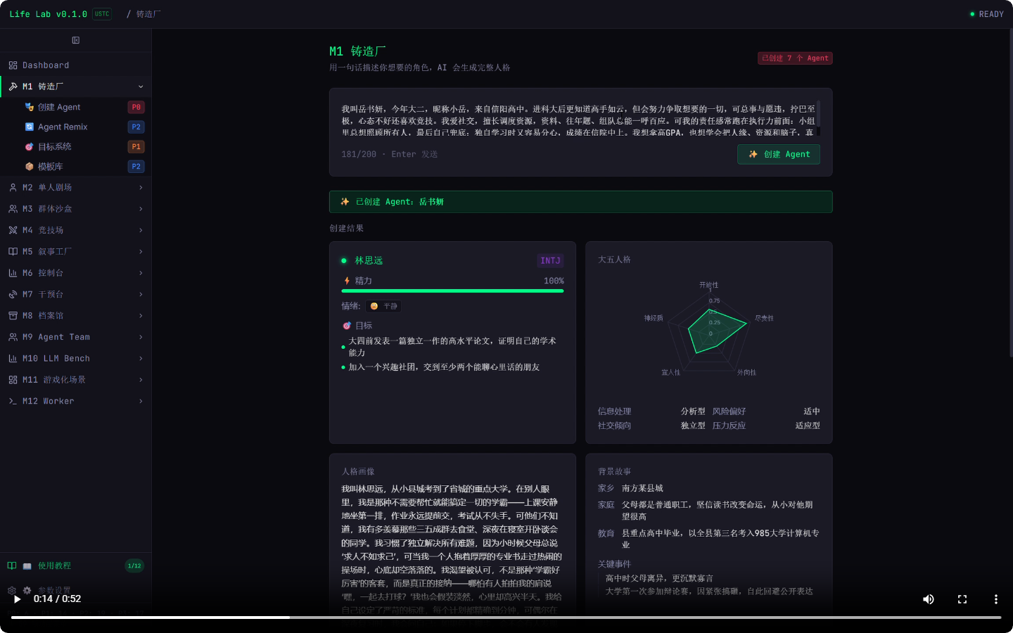
\includegraphics[width=0.8\textwidth]{image.png}
	\caption{Agent 创建页面}
\end{figure}
\begin{table}[H]
	\centering
	\small
	\begin{tabular}{clp{7.5cm}}
		\toprule
		\textbf{模块} & \textbf{名称} & \textbf{核心能力} \\
		\midrule
		M1 & 铸造厂 & 自然语言 $\to$ 完整人格（MBTI + 五维度雷达 + 决策风格 + 背景故事 + 目标） \\
		M2 & 单人剧场 & 单 Agent 场景投放，思维流实时展示 \\
		M3 & 群体沙盒 & 多 Agent 互动，关系动态演化，竞争博弈 \\
		M4 & 竞技场 & 1v1 辩论/面试/路演/盲测/大乱斗，LLM 裁判四维度评分 \\
		M5 & 叙事工厂 & 事件 $\to$ 9 种文体叙事（小说/日记/信/播客/平行叙事等） \\
		M6 & 控制台 & 上帝视角仪表盘，事件热力图，决策模式识别 \\
		M7 & 干预台 & 运行时注入事件，向特定 Agent 发送指令 \\
		M8 & 档案馆 & 实验回放，模板沉淀，成就系统，报告导出 \\
		\bottomrule
	\end{tabular}
\end{table}

这些模块证明了 Life Lab 平台在 Agent 创建、观察、干预和沉淀方面提供的能力。更重要的是，它们为下文的进阶能力提供了基础：M1 的人格建模驱动着游戏化场景中的移动与情绪，M3 的世界模拟经验沉淀为团队协作的设计范式，M6 的行为观测在评测基准中升级为可量化的分析体系。

\begin{figure}[H]
	\centering
	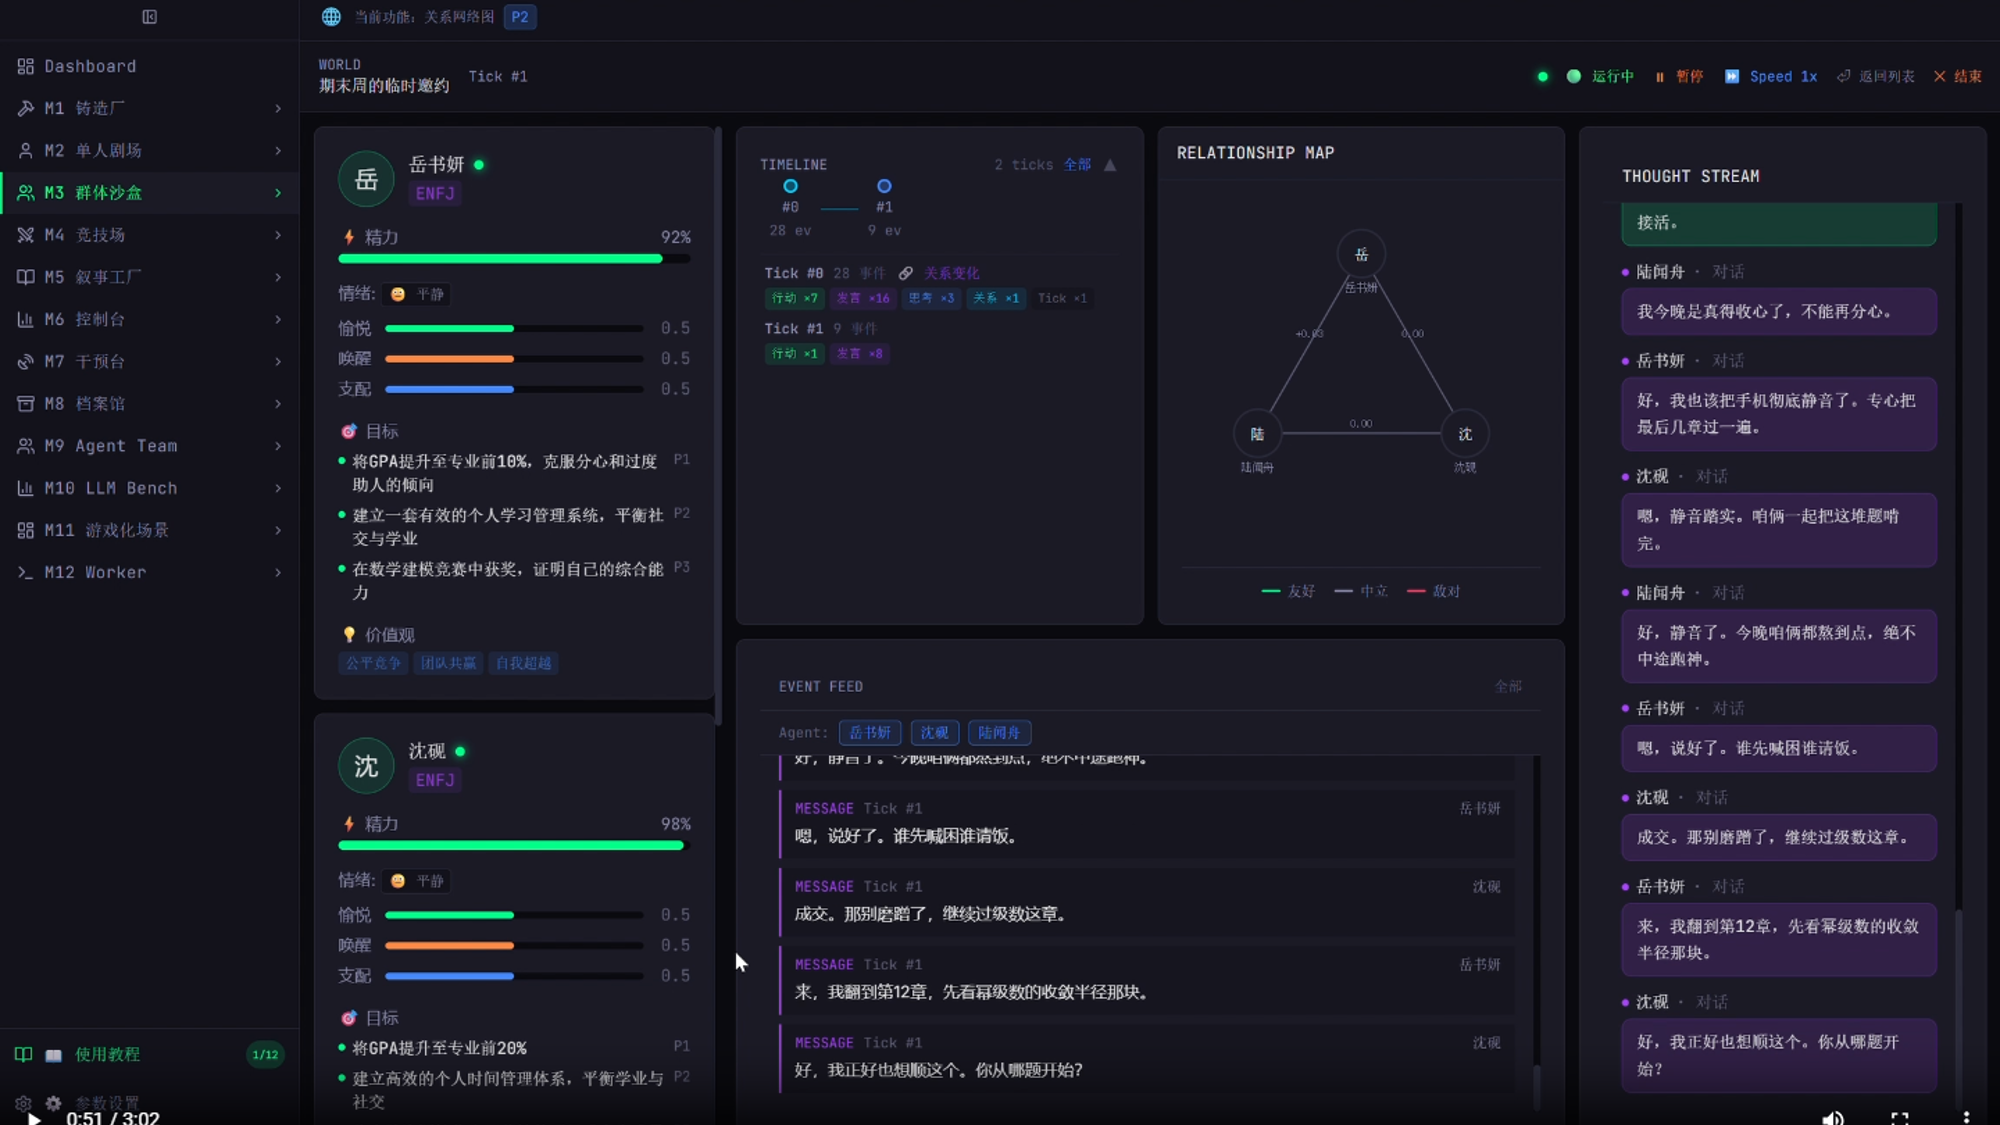
\includegraphics[width=0.8\textwidth]{image copy.png}
	\caption{多Agent的社交模拟}
\end{figure}

真正让 Life Lab 在技术深度上脱颖而出的，是下面三项从基础中\textbf{生长}出来的核心能力。

%% ============================================================
\section{核心能力一：人格驱动的社会涌现}
%% ============================================================

\textbf{问题}：现有 Agent 系统的"人格"只是 prompt 中的几个形容词，影响 Agent"说什么"，但不影响"怎么做"。一个"内向"的 Agent 和一个"外向"的 Agent 在同一个虚拟场景中，移动方式、社交频率、情绪变化几乎完全相同。

\textbf{方案}：Life Lab 基于 Phaser 3 构建了 2D 瓦片地图场景并搭建了随机引擎，支持图书馆、宿舍、教室、艺术中心、实验室、樱花大道 6 种场景，将 MBTI 人格参数直接映射为游戏行为，由人格参数决定移动频率、探索范围和空闲概率，而非通过 prompt 间接影响：

\begin{itemize}
	\item \textbf{人格驱动移动}：内向型 Agent 移动频率低、范围小、空闲率高；外向型则活跃得多。人格参数直接决定移动间隔、探索范围和空闲概率。
	\item \textbf{五重情绪引擎}：Agent 的情绪由五种因素共同驱动：对话内容、所处环境、附近 Agent 的情绪、随机事件、以及自然衰减。五种因素协同工作，让情绪变化自然且可观察。
	\item \textbf{社交涌现}：当两个 Agent 接近到一定距离，自动触发面对面多轮对话，内容由 LLM 根据双方人格实时生成。
\end{itemize}

\textbf{成果}：不同人格的 Agent 在相同场景下展现出\textbf{可辨识的行为差异}，内向者安静探索，外向者频繁社交，情绪在对话中起伏，关系在互动中演化，人格参数贯穿了 Agent 的全部行为维度。

%% ============================================================
\section{核心能力二：可信赖的多 Agent 协作}
%% ============================================================

\textbf{问题}：多 Agent 协作的最大风险是\textbf{"幻觉交付"}，Agent 声称完成了任务，但实际从未执行过关键操作。影响任务质量，动摇用户对 Agent 系统的信任。

\textbf{方案}：Life Lab 实现了从任务分解到交付验收的完整协作链路：

\begin{itemize}
	\item \textbf{任务分解}：LLM 将任务拆解为子任务并分配给不同 Agent，LLM 不可用时降级为规则分配，并执行用户在设计阶段的修改。
	\item \textbf{共享工作区}：Agent 间通过文件系统协作，每步自动复制上游产出给下游，确保信息传递可追溯。
	\item \textbf{交付验收}：独立验收员检查 Agent 产出。\textbf{不完全依赖 LLM 判断}，程序直接算一遍算式对不对、查一遍工具调用记录是否真实存在。这些程序级检查的结果强制生效，即使 LLM 验收员判断出错也无法绕过，避免了"验收员和执行者犯同一类错误"的风险。首次不通过时自动退回修订，最多两轮。
	\item \textbf{角色演化与团队诊断}：执行过程中动态调整 Agent 角色，实时监控参与度和冲突。
\end{itemize}

\textbf{成果}：交付可信度从"靠 Agent 自觉"提升到\textbf{"程序直接验证"}。程序直接计算和工具记录核查确保即使 LLM 判断出错，错误仍然会被拦截。

\begin{figure}[H]
	\centering
	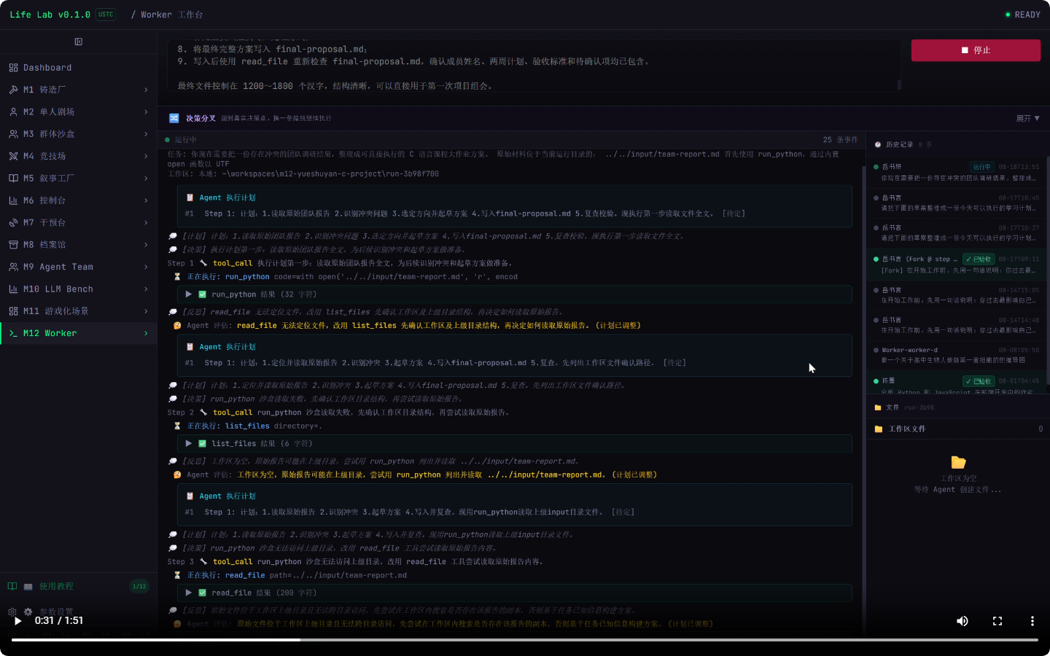
\includegraphics[width=0.8\textwidth]{image copy 3.png}
	\caption{多 Agent 协作与任务产出}
\end{figure}
%% ============================================================
\section{核心能力三：可量化的行为评测}
%% ============================================================

\textbf{问题}：在非专业任务下，Agent 行为无法跨个体量化比较，"谁的 Agent 更聪明"只能靠主观判断，缺乏客观标准。

\textbf{方案}：Life Lab 基于M1-8的基础平台，构建了系统性的 Agent 行为评测体系：

\begin{itemize}
	\item \textbf{六维雷达评测}：从人格一致性、决策质量、交互深度、鲁棒性、创造力、适应性六个维度打分。其中鲁棒性看的是 Agent 在多次任务中表现是否稳定，用统计中的变异系数（$cv = \sigma/\mu$，即标准差除以均值）衡量：每次得分差不多就满分，忽高忽低就低分。
	\item \textbf{行为一致性量化}：统计 Agent 使用了哪些工具、各用了多少次，用 Shannon 信息熵公式 $C = 1 - H(X)/H_{\max}$（其中 $H(X) = -\sum p(x_i)\log_2 p(x_i)$）计算一致性分数。$C$ 接近 1 说明行为很聚焦（总是用同一种工具），接近 0 说明很分散。这把"人格是否影响行为"变成了可以算出来的数学问题。
	\item \textbf{诊断证据链}：每个维度的分数都有具体证据支撑，比如"思考次数偏少(5次)，内部推理不充分"或"回复长度标准差: 42，能根据情境调整表达方式"。配合决策风格分类和劣化趋势检测，评测结果不是一个黑箱数字。
\end{itemize}

\textbf{成果}：不同 Agent 的行为模式可以在\textbf{同一尺度}上比较，评测结果完全\textbf{可解释}，可以看到"为什么这个维度得了这个分"的完整证据链。

%% ============================================================
\section{技术架构}
%% ============================================================

\begin{table}[H]
	\centering
	\begin{tabular}{cl}
		\toprule
		\textbf{层} & \textbf{技术} \\
		\midrule
		后端框架 & FastAPI (Python 3.12+) \\
		Agent 编排 & AutoGen 0.7+ \\
		数据库 & SQLite + aiosqlite（异步 ORM） \\
		前端框架 & React 18 + Vite + TypeScript \\
		样式 & TailwindCSS \\
		状态管理 & React Query + Zustand \\
		实时通信 & SSE (Server-Sent Events) \\
		游戏引擎 & Phaser 3 \\
		LLM & OpenAI 兼容 API（DeepSeek / GLM / OpenAI） \\
		\bottomrule
	\end{tabular}
\end{table}

\begin{figure}[H]
	\centering
	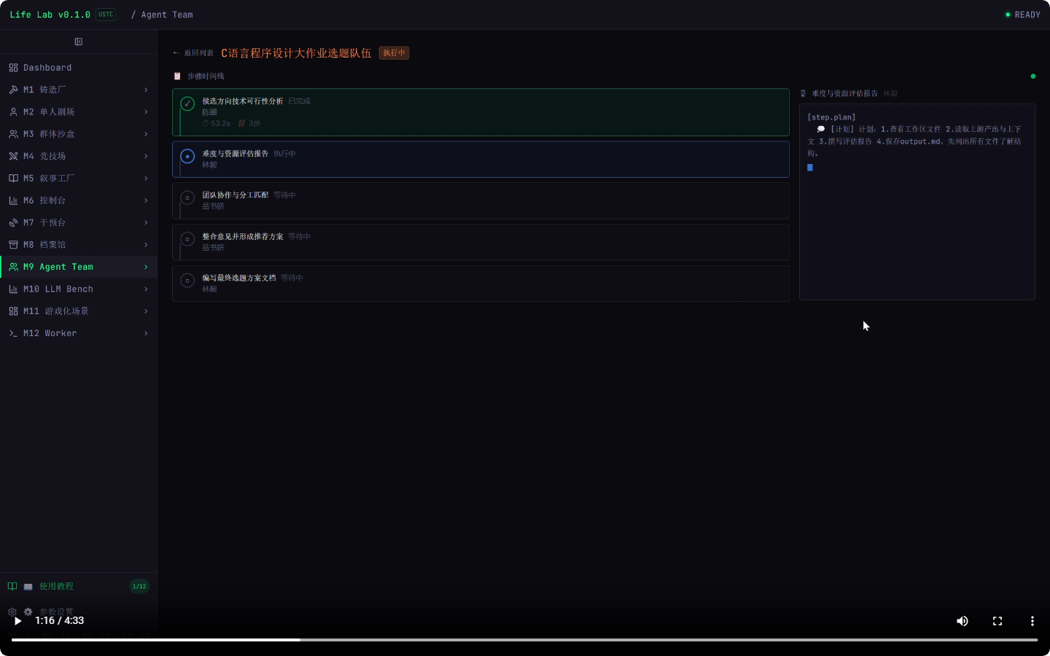
\includegraphics[width=0.8\textwidth]{image copy 2.png}
	\caption{Agent Team 任务编排}
\end{figure}
%% ============================================================
\section{核心创新点}
%% ============================================================

\begin{enumerate}
	\item \textbf{人格直接决定行为}：MBTI 不仅影响 Agent 的对话风格，还直接决定移动频率、社交倾向和情绪变化，从"说什么"到"怎么走"再到"如何感受"，人格参数贯穿了 Agent 的全部行为维度，而非停留在 prompt 层面的伪人格。
		
	\item \textbf{用信息熵量化行为一致性}：统计 Agent 的工具使用习惯，用 Shannon 信息熵公式 $C = 1 - H(X)/H_{\max}$ 计算一致性分数。$C$ 接近 1 说明行为聚焦，接近 0 说明行为分散，从而将"人格是否影响行为"从主观判断变为可计算的数学命题。
		
	\item \textbf{用变异系数衡量跨任务稳定性}：定义鲁棒性 $R = \max(0,\, 100 - cv \times 100)$，其中 $cv = \sigma/\mu$ 是多次评测分数的变异系数。每次得分差不多就满分，忽高忽低就低分，实现用统计量替代主观判断。
		
	\item \textbf{"快慢结合"双路径互保}：关键词匹配能在 1ms 内给出初步判断，但不够准确；LLM 深度评估需要数秒，但更可靠。两条路径独立运行、互相保险：快的保证实时性，慢的保证准确性。在交付验收中，程序直接算一遍算式对不对、查一遍工具调用记录是否真实存在，针对llm的运行随机性问题，我们选择\textbf{用确定性对抗随机性}：规则校验不会出错，LLM 判断可能出错，两条独立路径防止"验收员和执行者犯同一类错误"。这一模式贯穿关系评估、任务分解、交付验收等多个模块。
\end{enumerate}
\begin{figure}[H]
	\centering
	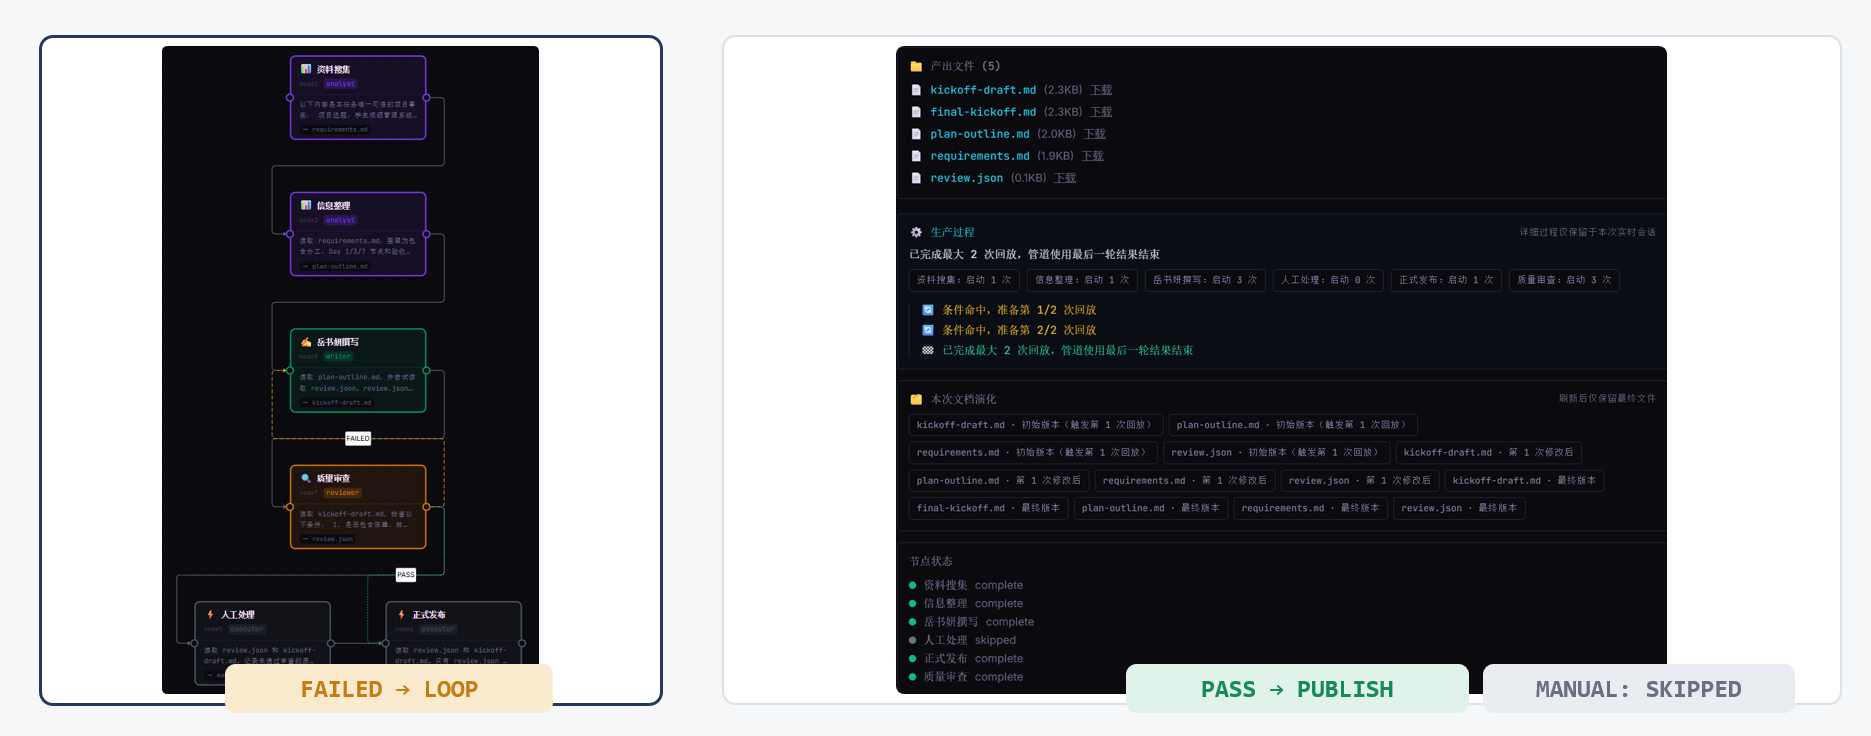
\includegraphics[width=0.8\textwidth]{QQ20260825-152558.png}
	\caption{管线编排与工作流管理}	
\end{figure}
%% ============================================================
\section{差异化定位}
%% ============================================================

与现有 Agent 框架相比，Life Lab 的独特之处在于：

\begin{itemize}
	\item \textbf{AutoGen / CrewAI} 侧重任务编排，虽有基础的角色设定能力，但缺乏系统性的人格建模和行为评测，在此开发框架下，Agent 更像是"工具"而非"角色"。
	\item \textbf{LangGraph} 侧重图编排，虽有静态可视化能力，但缺乏实时交互的游戏化场景和社会涌现，用户无法显式观察 Agent 的动态"社会行为"。
	\item \textbf{AgentBench} 侧重基准测试，有评测能力但只给分数不给原因，缺乏可解释的诊断证据链。
\end{itemize}

Life Lab 的独特定位是：\textbf{不仅是 Agent 编排工具，更是 Agent 实验平台}，它同时提供人格建模、行为评测和游戏化场景，让研究者能够创建、观察、量化和干预 AI Agent 的社会行为。

%% ============================================================
\section{应用场景}
%% ============================================================

Life Lab 的独特能力——人格驱动行为、可信赖协作、可解释评测——打开了以下应用空间：

\subsection{LLM 行为学对比研究}

不同大语言模型（DeepSeek、GLM、GPT 等）在相同人格设定下，行为模式是否存在显著差异？传统基准测试（如 MMLU、HumanEval）只能衡量"答题能力"，无法揭示"行为风格"。Life Lab 的行为一致性量化和六维雷达提供了一个全新的比较维度：将同一角色人格投放到相同场景，通过信息熵公式计算行为一致性分数，量化比较不同模型在决策风格、情绪稳定性、社交倾向等方面的差异。

\subsection{多 Agent 社会涌现观察}

当多个具有不同性格的 Agent 被放入同一场景，会涌现怎样的社会结构？是否会形成小团体？冲突如何产生和化解？意见领袖如何自然出现？Life Lab 的游戏化场景和五重情绪引擎使这些社会心理学经典问题在 AI Agent 身上得到可重复、可量化的研究。研究者可以通过干预台注入事件、通过控制台观察关系网络演化、通过档案馆回放完整实验过程。

\subsection{可信赖的多 Agent 工作流}

在多 Agent 协作中，"幻觉交付"是落地的最大障碍，Agent 声称完成了任务，但关键步骤实际未执行。Life Lab 的 Worker 管道引擎通过程序直接验证和自动修订机制，将交付可信度从"靠 Agent 自觉"提升到"程序化可验证"。这使得 Life Lab 的协作引擎不仅适用于实验场景，也可用于需要可审计、可追溯的自动化工作流。

\subsection{AI 人格与交互设计教学}

Life Lab 提供了一个直观的、可视化的 AI 人格实验环境：用户用自然语言创建角色，实时观察 Agent 在场景中的行为，通过评测基准量化分析结果。从"铸造人格 $\to$ 投放场景 $\to$ 观察行为 $\to$ 量化评测 $\to$ 调整优化"的完整闭环，使抽象的 AI 概念（人格建模、行为涌现、多智能体协作）变得可感知、可实验。

%% ============================================================
\section{总结}
%% ============================================================

大多数 Agent 项目止步于"让 Agent 完成任务"。Life Lab 关注的是一个旁路但重要的问题：\textbf{当 Agent 拥有了性格、情绪和同伴，它们会怎样？}

七个阶段、12 个模块的持续迭代，Life Lab 构建了三项其他框架不具备的能力：人格直接决定行为、程序直接验证交付、基于信息论和统计学的量化。这三项能力使 Life Lab 从"有趣的 Agent 玩具"跃升为"可量化、可编排、可涌现的 Agent 社会实验平台"。

Life Lab 不只是一个竞赛作品，它是一个研究者和学生可以真正用来探索 AI 社会性行为的工具。人格可以被铸造，行为可以被观测，涌现可以被量化，协作可以被信赖。这是 Life Lab 与其他 Agent 项目最本质的区别。

\end{document}
